%!TeX encoding = UTF-8
%!TEX TS-program = pdflatex
% Author: Phil Steinhorst, p.st@wwu.de
%!TEX root = thesis.tex
% Author: Phil Steinhorst, p.st@wwu.de

% **************************************************
% Document Class Definition
% **************************************************
\documentclass[%
	paper=A4,					% paper size --> A4 is default in Germany
	twoside=true,				% onesite or twoside printing
	openright,					% doublepage cleaning ends up right side
	parskip=full,				% spacing value / method for paragraphs
	chapterprefix=true,			% prefix for chapter marks
	10pt,						% font size
	headings=normal,			% size of headings
	bibliography=totoc,			% include bib in toc
	listof=totoc,				% include listof entries in toc
	titlepage=on,				% own page for each title page
	captions=tableabove,		% display table captions above the float env
	draft=false,				% value for draft version
]{scrreprt}%

% **************************************************
% Debug LaTeX Information
% **************************************************
%\listfiles

% **************************************************
% Information and Commands for Reuse
% **************************************************
\newcommand{\thesisTitle}{The Clean Thesis Style}
\newcommand{\thesisName}{Ricardo Langner}
\newcommand{\thesisSubject}{Documentation}
\newcommand{\thesisDate}{August 26, 2015}
\newcommand{\thesisVersion}{My First Draft}

\newcommand{\thesisFirstReviewer}{Jane Doe}
\newcommand{\thesisFirstReviewerUniversity}{\protect{Clean Thesis Style University}}
\newcommand{\thesisFirstReviewerDepartment}{Department of Clean Thesis Style}

\newcommand{\thesisSecondReviewer}{John Doe}
\newcommand{\thesisSecondReviewerUniversity}{\protect{Clean Thesis Style University}}
\newcommand{\thesisSecondReviewerDepartment}{Department of Clean Thesis Style}

\newcommand{\thesisFirstSupervisor}{Jane Doe}
\newcommand{\thesisSecondSupervisor}{John Smith}

\newcommand{\thesisUniversity}{\protect{Clean Thesis Style University}}
\newcommand{\thesisUniversityDepartment}{Department of Clean Thesis Style}
\newcommand{\thesisUniversityInstitute}{Institut for Clean Thesis Dev}
\newcommand{\thesisUniversityGroup}{Clean Thesis Group (CTG)}
\newcommand{\thesisUniversityCity}{City}
\newcommand{\thesisUniversityStreetAddress}{Street address}
\newcommand{\thesisUniversityPostalCode}{Postal Code}

% **************************************************
% Load and Configure Packages
% **************************************************
\usepackage[utf8]{inputenc}		% defines file's character encoding
\usepackage[ngerman]{babel} % babel system, adjust the language of the content
\usepackage[					% clean thesis style
	sansserif=false,%
	hangfigurecaption=false,%
	hangsection=true,%
	hangsubsection=true,%
	figuresep=colon,%
	colorize=full,%
	colortheme=bluemagenta,%
	bibsys=biber,%
	bibfile=bib-refs,%
	bibstyle=alphabetic,%
]{cleanthesis}

\hypersetup{					% setup the hyperref-package options
	pdftitle={\thesisTitle},	% 	- title (PDF meta)
	pdfsubject={\thesisSubject},% 	- subject (PDF meta)
	pdfauthor={\thesisName},	% 	- author (PDF meta)
	plainpages=false,			% 	-
	colorlinks=false,			% 	- colorize links?
	pdfborder={0 0 0},			% 	-
	breaklinks=true,			% 	- allow line break inside links
	bookmarksnumbered=true,		%
	bookmarksopen=true			%
}
\listfiles
\begin{document}

\listoftodos

%%% General ToDos %%%
\begin{enumerate}
	\item lokale/globale Variablen
	\item Pointer/Fields ohne Verweise auf \Roots
	\item $\Pointers, \Fields$
	\item Nochmal Bezeichnungen durchgehen
	\item Punkt-Verknüpfungen
	\item Transitive Hülle
	\item Übergänge zwischen Kapiteln
	\item Methode
	\item Bildungssprache
	\item Zeilenzahlen
	\item Seitenumbrüche, Verzeichnisse
\end{enumerate}

%!TEX root = ../../thesis.tex
% Author: Phil Steinhorst, p.st@wwu.de

% --------------------------
% Front matter
% --------------------------
\pagenumbering{roman}				% roman page numbing (invisible for empty page style)
\pagestyle{empty}					% no header or footers
% !TEX root = ../../thesis.tex
%
% ------------------------------------  --> cover title page
%\begin{titlepage}
%	\pdfbookmark[0]{Cover}{Cover}
%	\flushright
%	\hfill
%	\vfill
%	{\LARGE\thesisTitle \par}
%	\rule[5pt]{\textwidth}{.4pt} \par
%	{\Large\thesisName}
%	\vfill
%	\textit{\large\thesisDate} \\
%	Version: \thesisVersion
%\end{titlepage}


% ------------------------------------  --> main title page
\begin{titlepage}
	\pdfbookmark[0]{Titelblatt}{Titelblatt}
	\tgherosfont
	
	\begin{minipage}[b]{0.4\textwidth}
	\begin{flushleft}
	
\includegraphics[width=5.5cm,keepaspectratio]{img/wwulogo17.eps}\\[1cm]
	\end{flushleft}
	\end{minipage}
	\hfill
	\begin{minipage}[b]{0.5\textwidth}
	\begin{flushright}
	%\vspace*{0.45cm}
	\footnotesize
	Westfälische Wilhelms-Universität Münster \\
	Fachbereich 10 -- Mathematik und Informatik \\
	Institut für Informatik
%	\textsf{Westfälische Wilhelms-Universität Münster} \\
%	\textsf{Fachbereich 10 -- Mathematik und Informatik} \\
%	\textsf{Institut für Informatik}
	\end{flushright}
	\end{minipage}
		
	%{\Large \thesisUniversity} \\[4mm]
	%\includegraphics[width=6cm]{gfx/Clean-Thesis-Logo} \\[2mm]
	%\textsf{\thesisUniversityDepartment} \\
	%\textsf{\thesisUniversityInstitute} \\
	%\textsf{\thesisUniversityGroup} \\

	\vfill
	
	\centering
	
	{\large \thesisSubject} \\[5mm]
	{\huge \color{ctcolortitle}\textbf{Garbage-Collection-Algorithmen \\ und ihre Simulation} \\[10mm]}
	{\LARGE \thesisName}

	\vfill
	\begin{minipage}[t]{.4\textwidth}
		\raggedleft
		\textit{Erstgutachter und Betreuung}
	\end{minipage}
	\hspace*{15pt}
	\begin{minipage}[t]{.45\textwidth}
		{\Large \thesisFirstReviewer} \\
	  	%{\small \thesisFirstReviewerDepartment} \\[-1mm]
		%{\small \thesisFirstReviewerUniversity}
	\end{minipage} \\[0mm]
	\begin{minipage}[t]{.4\textwidth}
		\raggedleft
		\textit{Zweitgutachter}
	\end{minipage}
	\hspace*{15pt}
	\begin{minipage}[t]{.45\textwidth}
		{\Large \thesisSecondReviewer} \\
	  	%{\small \thesisSecondReviewerDepartment} \\[-1mm]
		%{\small \thesisSecondReviewerUniversity}
	\end{minipage} \\[10mm]
%	\begin{minipage}[t]{.27\textwidth}
%		\raggedleft
%		\textit{Betreuung}
%	\end{minipage}
%	\hspace*{15pt}
%	\begin{minipage}[t]{.65\textwidth}
%		\thesisFirstSupervisor\ and \thesisSecondSupervisor
%	\end{minipage} \\[10mm]

	\thesisAuthorCity, \thesisDate \\

\end{titlepage}


% ------------------------------------  --> lower title back for single page layout
\hfill
\vfill
{
	\small
	\textbf{\thesisTitle} \\
	\thesisSubject\ zur Erlangung des akademischen Grades \textit{\thesisDegree} \\
	in den Fächern \thesisAuthorFirstSubject\ und \thesisAuthorSecondSubject \\
	Erstgutachter und Betreuung: \thesisFirstReviewer \\
	Zweitgutachter: \thesisSecondReviewer \\
%	Betreuung: \thesisFirstSupervisor\ und \thesisSecondSupervisor \\
	\thesisAuthorCity, \today \\[1.5em]	
	\textbf{\thesisName} \\
	\thesisAuthorStreet, \thesisAuthorPostalCode\ \thesisAuthorCity \\
	\texttt{\thesisAuthorMail} \\
	Matrikelnummer: \thesisAuthorId \\[1.5em]
	\textbf{\thesisUniversity} \\
	\thesisUniversityDepartment \\
	\thesisUniversityInstitute \\
	\thesisUniversityStreetAddress, \thesisUniversityPostalCode\ \thesisUniversityCity
}
		% INCLUDE: all titlepages
\cleardoublepage

\pagestyle{plain}					% display just page numbers
% !TEX root = ../../thesis.tex
%
\pdfbookmark[0]{Zusammenfassung}{Zusammenfassung}
\chapter*{Zusammenfassung}
\label{sec:abstract}
\vspace*{-10mm}

Die vorliegende Arbeit soll eine Aufarbeitung verschiedener Ansätze für Garbage-Collection-Algorithmen liefern.
Nach einer kurzen Darstellung der zugrunde liegenden Problematik und deren praktische Relevanz sowie den Vor- und Nachteilen einer automatischen Speicherverwaltung gegenüber einer manuellen Speicherverwaltung werden gängige Ansätze vergleichend vorgestellt sowie Einsatz und Eignung in der Praxis beurteilt.
Als Gütekriterien dienen hier beispielsweise Laufzeitbetrachtungen, Speicherbedarf und entstehende Verzögerungen im Programmablauf, die für ausgewählte Ansätze besonders detailliert untersucht werden.

Weiter wird eine Anwendung entworfen, mit der die Arbeitsweise der diskutierten Garbage-Collection-Ansätze visualisiert werden kann.
Dazu gehört eine angemessene Visualisierung eines beschränkten Speicherbereichs, etwa durch eine optische Unterscheidbarkeit belegter Blöcke, sowie der einzelnen Arbeitsphasen, die eine Garbage Collection ausführt.
Dabei sollen auch unterschiedliche Szenarien auswählbar sein, etwa verschiedene Speicherfüllstände und eine variable Anzahl bzw. Größe von Objekten, die im Speicher hinterlegt sind.

\todo[inline]{Am Ende nochmal schauen, ob das wirklich so ist :D}

\vspace*{20mm}

{\usekomafont{chapter}Abstract}\label{sec:abstract-diff} \\
\todo[inline]{Englisch einfügen.}		% INCLUDE: the abstracts (english and german)
\cleardoublepage

\setcounter{tocdepth}{2}		% define depth of toc
\tableofcontents				% display table of contents

\cleardoublepage

\pagenumbering{arabic}
\setcounter{page}{1}
\pagestyle{maincontentstyle}

% !TEX root = ../thesis.tex
\chapter{Einleitung}
\label{cha:intro}

\todo[inline]{Einleitung: Was ist Garbage Collection, wozu ist das relevant?}

\cite{mccarthy}

\section{Problemstellung und Terminologie}
\label{sec:intro:problem}

\todo[inline]{Was ist das Ziel einer GC? Wie kann man das möglichst formal ausdrücken? Grundbegriffe und Modellierung des Speichers?}
\part{Algorithmen und Ansätze}
%!TEX root = ../../thesis.tex
\chapter{Mark and Sweep}
\label{cha:mark-sweep}
Wir beginnen mit einer Vorstellung des ersten Garbage-Collection-Algorithmus, der auf John \textsc{McCarthy} zurückgeht \cite[191--193]{mccarthy1960}.
Im Rahmen eines im Jahr 1960 veröffentlichten Artikels über die Berechnung rekursiver Funktionen auf dem \textit{IBM 704} mithilfe des \textit{LISP Programming Systems} erläutert McCarthy die Speicherung von Daten in einer Listenstruktur.
Diese besteht aus Paaren, deren erster Eintrag \texttt{car} die zu speichernde Information enthält, während im zweiten Eintrag \texttt{cdr} die Registeradresse des nachfolgenden Paares zu finden ist.
Register, die aktuell nicht zur Speicherung von Daten genutzt werden, befinden sich in einer \textit{free storage list}.
Bei der Anforderung von Speicher für ein zu speicherndes Datum werden Register aus dieser Liste entfernt.
Durch die Manipulation der Registeradressen können Paare verwaisen, was zu Speicherlecks führt.
Zur Auflösung dieser Problematik bietet LISP als erste Programmiersprache ihrer Zeit eine automatische Speicherverwaltung, die von McCarthy wie folgt grob umschrieben wird:
Im Falle von Speicherknappheit wird -- ausgehend von einer Menge von Basisregistern -- ermittelt, welche Register über eine Folge von \texttt{cdr}-Einträgen erreichbar sind.
Nicht erreichbare Register enthalten überschreibbare Inhalte, sodass diese zurück in die \textit{free storage list} eingefügt werden können und wieder als freie Speicherplätze zu Verfügung stehen.
Diese zweischrittige Vorgehensweise -- das Erkennen nicht mehr benötigter Speicherbereiche und die anschließende Freigabe eben jener -- bildet die Grundlage des \textit{Mark-and-Sweep}-Algorithmus.

\section{Naives Mark and Sweep}
\label{sec:naive-mark-sweep}
Der naive Mark-and-Sweep-Algorithmus arbeitet in zwei Schritten:
Zunächst wird bestimmt, welche Objekte im Speicher unerreichbar sind, weil sie von keinem anderen erreichbaren Objekt referenziert werden.
Diese Objekte können gefahrlos freigegeben werden, da auf ihre Informationen nicht mehr zugegriffen werden kann.
Der zweite Schritt besteht aus einer Traversierung des gesamten Heaps.
Dabei werden alle existierenden Objekte besucht und diejenigen freigegeben, die im ersten Schritt als unerreichbar identifiziert werden konnten.
Die entsprechenden Speicherbereiche stehen anschließend wieder für neue Objekte zu Verfügung.

\begin{algorithm}
\begin{algorithmic}[1]
	\State \MethodHead{collectGarbage}():
	\State \quad \Method{markStart}()
	\State \quad \Method{sweepHeap}()
	\State
	\State \MethodHead{markStart}():
	\State \quad \Var{toDo} $\gets$ $\emptyset$				\Comment{Noch abzuarbeitende Objekte}
	\State \quad \FOREACH \Var{obj} $\in \Roots$		\Comment{Beginne mit Basisobjekten}
	\State \quad \quad \IF \Method{isNotMarked}(\Var{obj})
	\State \quad \quad \quad \Method{setMarked}(\Var{obj})	\Comment{Objekt als erreichbar markieren}
	\State \quad \quad \quad \Method{add}(\Var{toDo}, \Var{obj})	
	\State \quad \quad \quad \Method{mark}()			\Comment{Abarbeitung starten}
	\State
	\State \MethodHead{mark}():
	\State \quad \WHILE \Var{toDo} $\neq \emptyset$
	\State \quad \quad \Var{obj} $\gets$ \Method{remove}(\Var{toDo})			\Comment{Hole nächstes Objekt}
	\State \quad \quad \FOREACH \Var{adr} $\in \Pointers(\Var{obj})$	\Comment{Hole nächste Referenz auf Objekt}
	\State \quad \quad \quad \IF (\Var{adr} $\neq$ \Null $\wedge$ \Method{isNotMarked}(\Var{*adr}))	
	\State \quad \quad \quad \quad \Method{setMarked}(\Var{*adr})	
	\State \quad \quad \quad \quad \Method{add}(\Var{toDo}, \Var{*adr})
\end{algorithmic}
\caption[Naives Mark and Sweep -- Markierung]{Naives Mark and Sweep -- Markierung (vgl. \cite[Kap. 2.2]{jones-lins})}
\label{algo:naive-mark}
\end{algorithm}

Die Markierungsphase (engl. \textit{mark}) funktioniert wie folgt:
Zunächst wird mittels der Methode \Method{markStart} eine Menge \Var{toDo} erzeugt, die diejenigen Objekte enthält, die bereits als erreichbar erkannt wurden, aber selbst noch nicht verarbeitet wurden (Zeile 6 in Algorithmus~\ref{algo:naive-mark}).
In diese werden alle bislang unmarkierten Basisobjekte der Menge \Roots eingefügt und markiert, da sie in jedem Fall erreichbar sind (Zeile 7 bis 10).
Ist ein Basisobjekt bereits markiert worden, so wurde es schon entdeckt -- etwa, weil es durch ein zuvor abgearbeitetes Objekt referenziert wird.
Daraus folgt, dass es ebenfalls bereits abgearbeitet wurde oder sich noch in der Menge \Var{toDo} befindet.
In beiden Fällen muss es folglich nicht erneut zu \Var{toDo} hinzugefügt werden.

Bereits nach dem Hinzufügen des ersten Basisobjekts wird die Methode \Method{mark} aufgerufen, welche die \Var{toDo}-Menge abarbeitet.
Für jedes Objekt in \Var{toDo} werden diejenigen Felder betrachtet, die eine Referenz auf ein Objekt enthalten (Zeile 15 und 16).
Wenn dieses Objekt noch nicht markiert wurde, wird es in diesem Augenblick zum ersten Mal entdeckt.
Da es somit erreichbar ist, kann es markiert und zu \Var{toDo} hinzugefügt werden, um zu einem späteren Zeitpunkt abgearbeitet zu werden (Zeile 17 und 18).
Verweist die Referenz hingegen auf ein Objekt, das bereits markiert wurde, wurde dieses schon zuvor entdeckt.
Auch hier ist ein erneutes Hinzufügen zu \Var{toDo} überflüssig.
Sobald \Var{toDo} leer ist, erfolgt die Rückkehr zur Methode \Method{markStart}, sodass ggfs. das nächste Basisobjekt abgearbeitet wird.

\todo[inline]{Kleines Beispiel hier, großes in den Anhang?}

Es ist wesentlich, dass Objekte bereits markiert werden, wenn sie der Menge \Var{toDo} hinzugefügt werden, und nicht etwa, nachdem sie abgearbeitet wurden (Zeile 9 und 10 bzw. 18 und 19).
Andernfalls besteht bei zyklischen Referenzen die Gefahr einer Endlosschleife, da unmarkierte Objekte mehrfach hinzugefügt würden.
Präziser können wir festhalten, dass \Var{toDo} zu jedem Zeitpunkt ausschließlich bereits markierte Objekte enthält.
Da keine Objekte hinzugefügt werden, die bereits markiert wurden (Zeile 8 und 16), wird kein Objekt doppelt verarbeitet.
Da zudem mit jeder Iteration der \WHILE-Schleife mindestens ein Objekt aus \Var{toDo} entfernt wird (Zeile 15), die Anzahl aller Objekte endlich ist und wir voraussetzen, dass während der Ausführung des Garbage Collectors keine neuen Objekte entstehen, wird sowohl die \WHILE-Schleife, als auch die \FOREACH-Schleife nach endlich vielen Schritten terminieren.

Anstatt die Abarbeitung der \Var{toDo}-Menge zu beginnen, sobald das erste Basisobjekt erfasst wurde, können statt dessen auch zunächst alle Basisobjekte zu \Var{toDo} hinzugefügt und die Methode \Method{mark} im Anschluss aufgerufen werden.
Je nachdem, wie \Var{toDo} in der Praxis realisiert wird -- zum Beispiel in Form eines Stacks -- kann damit die Traversierung der Objekte beeinflusst werden.
Dies kann einen erheblichen Einfluss auf die Performanz der Markierungsphase haben, wenn Caching-Effekte eine Rolle spielen. \todo{evtl. später genauer drauf eingehen}

\begin{algorithm}
\begin{algorithmic}[1]
	\State \MethodHead{sweep}():
	\State \quad \Var{pos} $\gets$ \Method{nextObject}(\Var{HEAP\_START})
	\State \quad \WHILE \Var{pos} $\neq$ \Null
	\State \quad \quad \IF \Method{isMarked}(\Var{*pos})
	\State \quad \quad \quad \Method{unsetMarked}(\Var{*pos})
	\State \quad \quad \ELSE \Method{free}(\Var{pos})
	\State \quad \quad \Var{pos} $\gets$ \Method{nextObject}(\Var{pos})
\end{algorithmic}
\caption[Naives Mark and Sweep -- Bereinigung]{Naives Mark and Sweep -- Bereinigung (vgl. \cite[Kap. 2.2]{jones-lins})}
\label{algo:naive-sweep}
\end{algorithm}

Die Bereinigungsphase (engl. \textit{sweep}) beginnt unmittelbar nach der Markierungsphase durch Aufruf der Methode \Method{sweep}.
Die Variable \Var{pos} wird mit der Speicheradresse initialisiert, an der sich das erste Objekt im Heap befindet.
Wir gehen davon aus, dass eine Methode \Method{nextObject} zu Verfügung steht, die anhand einer übergebenen Speicheradresse die Adresse des nachfolgenden Objektes oder \Null zurückgibt, wenn dieses nicht existiert.
Dadurch wird der Heap linear traversiert; nicht markierte Objekte werden freigegeben, während die Markierung erreichbarer Objekte zurückgesetzt wird.

Wir halten zunächst fest, dass der Mark-and-Sweep-Algorithmus in seiner Gänze terminiert und korrekt ist, sofern während der Garbage Collection das laufende Programm angehalten wird:

\begin{mybox}
\begin{satz}
	\label{satz:mark-sweep-correctness}
	Der Mark-and-Sweep-Algorithmus terminiert und ist korrekt, wenn der Mutator während der Arbeit des Kollektors angehalten wird.
\end{satz}
\end{mybox}

\begin{proof}
	Wie oben erläutert, terminiert die Markierungsphase in jedem Fall, da bei angehaltenem Mutator keine neuen Objekte erstellt werden.
	Gleiches gilt für die Bereinigungsphase, in der alle Objekte des Heaps in endlicher Zeit besucht werden.
	Somit terminiert der gesamte Algorithmus.
	
	Weiter werden lediglich nicht markierte Objekte freigegeben (Zeile 4--6 in Algorithmus~\ref{algo:naive-sweep}).
	Bleibt ein Objekt \code{obj} unmarkiert, so ist \code{obj} kein Basisobjekt, da \Method{markStart} alle Basisobjekte markiert.
	Somit wird kein Basisobjekt freigegeben.
	Wir zeigen, dass es nach der Markierungsphase zudem keine zwei Objekte $\Var{a}$, $\Var{b}$ mit $\Var{a} \rightarrow \Var{b}$ gibt, sodass $\Var{a}$ markiert und $\Var{b}$ unmarkiert ist:
	Da $\Var{a}$ markiert ist, wurde $\Var{a}$ auch der Menge $\Var{toDo}$ hinzugefügt (Zeile 9f bzw. 18f in Algorithmus~\ref{algo:naive-mark}).
	Entsprechend gab es eine Iteration der \WHILE-Schleife mit $\Var{obj} = \Var{a}$.
	Gilt nun \Var{a} $\rightarrow$ \Var{b}, so ist $\Var{\&b} \in \Pointers(\Var{a})$.
	Folglich wird in einer Iteration der \FOREACH-Schleife mit \Var{adr} $=$ \Var{\&b} auch \Var{*(\&b)} $=$ \Var{b} markiert, falls \Var{b} nicht schon zuvor markiert wurde.
	Es existiert somit keine Referenz von einem erreichbaren auf ein unmarkiertes Objekt, weswegen keine erreichbaren Objekte freigegeben werden.
\end{proof}

Die Bedingung, dass der Mutator während des Markierens pausiert wird, ist tatsächlich notwendig, um zu vermeiden, dass fälschlicherweise keine erreichbaren Objekte entfernt werden, wie folgendes Beispiel zeigt (vgl. \cite[969]{dijkstra1978}):
Betrachten wir etwa die Situation, dass zwei Basisobjekte $\Var{A}$ und $\Var{B}$ alternierend auf ein Objekt $\Var{C}$ verweisen, das ausschließlich über $\Var{A}$ oder $\Var{B}$ erreichbar ist.
Während der Kollektor aktiv ist, führe der Mutator folgenden Code aus:

\begin{center}
\begin{minipage}{0.3\textwidth}
	\centering
	\begin{algorithmic}[1]
		\State \Var{B.ref} $\gets$ \Var{\&C}
		\State \Var{A.ref} $\gets$ \Null
		\State \Var{A.ref} $\gets$ \Var{\&C}
		\State \Var{B.ref} $\gets$ \Null
	\end{algorithmic}
\end{minipage}~
\begin{minipage}{0.3\textwidth}
	\centering
	\includegraphics[keepaspectratio]{img/tikz/ch2-concurrent1.pdf}
\end{minipage}~
\begin{minipage}{0.3\textwidth}
	\centering
	\includegraphics[keepaspectratio]{img/tikz/ch2-concurrent2.pdf}
\end{minipage}
\end{center}

Es könnte passieren, dass der Kollektor gerade Objekt $\Var{A}$ abarbeitet, unmittelbar nachdem Zeile~2 ausgeführt wurde.
Es wird dann keine Referenz auf Objekt $\Var{C}$ vorgefunden.
Wenn der Kollektor nun Objekt $\Var{B}$ betrachtet, nachdem bereits Zeile~4 abgearbeitet wurde, wird Objekt $\Var{C}$ weiterhin nicht entdeckt.
Insgesamt wird Objekt $\Var{C}$ somit nicht markiert, obwohl es erreichbar ist.
In der Folge würde $\Var{C}$ irrtümlich freigegeben werden, sodass im schlimmsten Fall ein hängender Zeiger entsteht oder sogar Datenverlust verursacht wird -- der Algorithmus arbeitet also nicht korrekt.

Algorithmen, die zur Vermeidung von \textit{race conditions} zwischen Kollektor und Mutator die Arbeit des letzteren unterbrechen, werden auch als \textit{Stop-the-World-Algorithmen} bezeichnet.

\section{Markierungsmöglichkeiten}
\label{sec:marking-methods}

\section{Drei-Farben-Abstraktion}
\label{sec:tricolor}
Da das Anhalten des Mutators während eines gesamten Garbage-Collection-Zyklus zu vergleichsweise großen Verzögerungen führt, ist eine Optimierung der Markierungsphase zielführend.
Wünschenswert ist, Kollektor und Mutator möglichst häufig eine nebenläufige Ausführung zu ermöglichen, ohne dabei die Korrektheit der Garbage Collection zu gefährden.
Wir haben gesehen, dass die Manipulation von Referenzen während der Markierungsphase dazu führt, dass Verweise von markierten auf unmarkierte Objekte entstehen können, sodass erreichbare Objekte unmarkiert bleiben.
Um dies zu vermeiden, könnte man als ersten Ansatz auf die Idee kommen, beim Schreiben einer neuen Referenz in ein Feld eines Objekts das Ziel dieser Referenz sofort zu markieren.
Dies ist jedoch nur scheinbar eine Lösung:
Da das Ziel ebenfalls Referenzen auf unmarkierte Objekte bereithalten könnte, entstehen dadurch möglicherweise neue Referenzen von markierten auf unmarkierte Objekte.
Von Dijkstra et al. stammt ein Ansatz, der diese Idee aufgreift und um ein \textit{Zwischenstadium} erweitert \cite[S. 969f]{dijkstra1978}.
Diese ermöglicht es, markierte Objekte, die bereits komplett abgearbeitet wurden, von solchen zu unterscheiden, die bislang lediglich entdeckt wurden.
Dazu werden Objekte mit drei verschiedenen Farben markiert:

\begin{description}
	\item[weiß:] Das Objekt wurde bislang nicht als erreichbar identifiziert.
		Bleibt es nach Ende der Markierungsphase weiß, kann es freigegeben werden.
	\item[grau:] Das Objekt ist erreichbar, allerdings wurden die Felder des Objekts noch nicht auf Referenzen zu weiteren Objekten überprüft.
	\item[schwarz:] Das Objekt ist erreichbar und alle Felder des Objekts wurden bereits überprüft.
\end{description}

Zu Beginn des Algorithmus sind alle existierenden Objekte weiß.
Wir modifizieren den ursprünglichen Mark-and-Sweep-Algorithmus~\ref{algo:naive-mark} so, dass Objekte bei ihrer Entdeckung grau und nach Abarbeitung ihrer Felder schwarz markiert werden.
Hierfür existiert eine atomare Prozedur \Method{setColor}, die die Markierung eines Objekts auf eine bestimmte Farbe \Var{WHITE}, \Var{GRAY} oder \Var{BLACK} setzt.
Auf diese Art bleiben nicht mehr erreichbare Objekte weiß und können anschließend als löschbar identifiziert werden.
Analog wird die \Method{sweep}-Prozedur in Algorithmus~\ref{algo:naive-sweep} so abgeändert, dass Objekte gelöscht werden, wenn sie weiß markiert sind.
Andernfalls wird ihre Markierung zurück auf weiß gesetzt.

\begin{algorithm}[h]
\begin{algorithmic}[1]
	\Pre Alle Objekte sind weiß markiert.
	\State \MethodHead{markStart}():
	\State \quad \Var{graySet} $\gets$ $\emptyset$				\Comment{Grau markierte Objekte}
	\State \quad \FOREACH \Var{obj} $\in \Roots$
	\State \quad \quad \IF \Method{isWhite}(\Var{obj})
	\State \quad \quad \quad \Method{setColor}(\Var{obj}, \Var{GRAY})	
	\State \quad \quad \quad \Method{add}(\Var{graySet}, \Var{obj})	
	\State \quad \quad \quad \Method{mark}()
	\Statex
	\State \MethodHead{mark}():
	\State \quad \WHILE \Var{graySet} $\neq \emptyset$
	\State \quad \quad \Var{obj} $\gets$ \Method{remove}(\Var{graySet})
	\State \quad \quad \Method{setColor}(\Var{obj}, \Var{BLACK})		\Comment{Objekt wird nun abgearbeitet}
	\State \quad \quad \FOREACH \Var{adr} $\in \Pointers(\Var{obj})$
	\State \quad \quad \quad \IF (\Var{adr} $\neq$ \Null $\wedge$ \Method{isWhite}(\Var{*adr}))	
	\State \quad \quad \quad \quad \Method{setColor}(\Var{*adr}, \Var{GRAY})	\Comment{Referenzierte Objekte grau markieren}
	\State \quad \quad \quad \quad \Method{add}(\Var{graySet}, \Var{*adr})
	\Statex
	\State \MethodHead{sweep}():
	\State \quad \Var{pos} $\gets$ \Method{nextObject}(\Var{HEAP\_START})
	\State \quad \WHILE \Var{pos} $\neq$ \Null
	\State \quad \quad \IF \Method{isWhite}(\Var{*pos})
	\State \quad \quad \quad \Method{free}(\Var{pos})
	\State \quad \quad \ELSE \Method{setColor}(\Var{*pos}, \Var{WHITE})
	\State \quad \quad \Var{pos} $\gets$ \Method{nextObject}(\Var{pos})
\end{algorithmic}
\caption[Markierung mit Drei-Farben-Abstraktion]{Markierung mit Drei-Farben-Abstraktion (vgl. \cite[S. 970]{dijkstra1978})}
\label{algo:tricolor}
\end{algorithm}

Mithilfe dieser \textbf{Drei-Farben-Abstraktion} (engl. \textit{tri-color abstraction}) können wir nun Referenzmanipulationen zulassen, die parallel zur Markierungsphase der Garbage Collection stattfinden:
Wird in einem Objekt \Var{a} eine Referenz auf ein Objekt \Var{b} hinterlegt, so kann dies dazu führen, dass \Var{b} erreichbar wird.
Infolgedessen müssen auch alle von \Var{b} referenzierten Objekte als erreichbar identifiziert werden.
Somit ist es zielführend, \Var{b} beim Setzen der Referenz grau zu markieren und zu \Var{graySet} hinzuzufügen, sofern dies noch nicht der Fall ist oder die Felder von \Var{b} bereits verfolgt wurden.
Dies kann etwa mit einer \textit{Schreibbarriere} (engl. \textit{write barrier}) realisiert werden, die genau dann zum Einsatz kommt, wenn eine Referenz in ein Feld eines Objektes geschrieben wird (siehe Algorithmus~\ref{algo:tricolor-barrier}).
Auf diese Art kann es jedoch vorkommen, dass Objekte unerreichbar werden, nachdem sie bereits grau oder schwarz markiert wurden.
Entsprechend verbleiben sie zunächst im Speicher und werden erst im nächsten Garbage-Collection-Zyklus entfernt.

\begin{algorithm}[h]
\begin{algorithmic}[1]
	\Input Objekt \Var{obj}, in dem Referenz gesetzt wird; Index des Feldes \Var{i}; zu setzende Referenz \Var{ref}
	\State \Atomic \MethodHead{writeRef}(\Var{obj}, \Var{i}, \Var{ref}):
	\State \quad \IF (\Var{ref} $\neq$ \Null $\wedge$ \Method{isWhite}(\Var{*ref}))
	\State \quad \quad \Method{setColor}(\Var{*ref}, \Var{GRAY})
	\State \quad \quad \Method{add}(\Var{grayList}, \Var{*ref})
	\State \quad \Var{obj[i]} $\gets$ \Var{ref}
\end{algorithmic}
\caption[Schreibbarriere zur Manipulation von Referenzen]{Schreibbarriere zur Manipulation von Referenzen in Objekten.}
\label{algo:tricolor-barrier}
\end{algorithm}

An dieser Stelle gehen wir auf die Terminierung und Korrektheit des modifizierten Mark-and-Sweep-Algorithmus ein.

\begin{mybox}
\begin{satz}
	Der Mark-and-Sweep-Algorithmus mit Drei-Farben-Abstraktion terminiert und ist korrekt, sofern während der Arbeit des Kollektors keine neuen Objekte erzeugt werden.
\end{satz}
\end{mybox}

\begin{proof}
	\textit{Zur Terminierung:} Wir halten zunächst fest, dass Objekte während der Markierungsphase ausschließlich \textit{dunkler} gefärbt werden:
	In Algorithmus~\ref{algo:tricolor} werden lediglich weiß markierte Objekte grau gefärbt (Zeile~5 und 14); eine Weißfärbung geschieht in dieser Phase grundsätzlich nicht.
	Analog zum ursprünglichen Algorithmus~\ref{algo:naive-mark} enthält \Var{graySet} nur grau markierte Objekte.
	Jedes Objekt befindet sich dadurch höchstens einmal in dieser Menge.
	Da \Var{graySet} nach jeder Iteration der \WHILE-Schleife um ein Objekt reduziert wird und keine neuen Objekte erzeugt werden, terminieren auch hier \WHILE- und \FOREACH-Schleife nach endlich vielen Schritten.
	Zuletzt terminiert auch Bereinigungsphase (siehe Satz~\ref{satz:mark-sweep-correctness}).
	
	\textit{Zur Korrektheit:} Erneut ist zu zeigen, dass keine Objekte unmarkiert bleiben, die erreichbar sind.
	Dies wäre genau dann der Fall, wenn nach der Markierungsphase ein schwarz markiertes Objekt eine Referenz auf ein weiß markiertes Objekt besitzt.
	Wir zeigen daher die Gültigkeit folgender Schleifeninvariante für die \WHILE-Schleife:
	\begin{description}
		\item[(A)] Es existieren keine zwei Objekte \Var{a} und \Var{b} mit \Var{a} $\rightarrow$ \Var{b}, sodass \Var{a} schwarz markiert und \Var{b} weiß markiert ist.
	\end{description}
	Da zu Beginn laut Vorbedingung alle Objekte weiß markiert sind und bis zum Eintritt in die \WHILE-Schleife Objekte nur grau markiert werden, gilt (A) trivialerweise, da keine schwarz markierten Objekte existieren.
	Gelte nun (A) zu Beginn einer Schleifeniteration und sei \Var{a} dasjenige Objekt, das der Menge \Var{graySet} entnommen und schwarz gefärbt wird (Zeile~10f).
	Existiert nun ein weiteres Objekt \Var{b} mit \Var{a} $\rightarrow$ \Var{b}, so ist \Var{\&b} $\in \Pointers(\Var{a})$.
	Ist \Var{b} bereits grau oder schwarz markiert, so geschieht nichts.
	Andernfalls wird \Var{*(\&b)} $=$ \Var{b} grau markiert (Zeile~14).
	In beiden Fällen ist \Var{b} am Ende der Schleife nicht weiß markiert.
	Da \Var{a} das einzige Objekt ist, das in dieser Iteration schwarz gefärbt wird, ist (A) nach der Iteration weiterhin gültig.
	Da die Schleife terminiert, die Invariante aufrecht erhalten bleibt und in der Bereinigungsphase nur weiß markierte Objekte freigegeben werden, ist der Algorithmus korrekt.
\end{proof}

Die Atomizität der Schreibbarriere \Method{writeRef} in Algorithmus~\ref{algo:tricolor-barrier} ist in der Tat notwendig, um die Korrektheit zu gewährleisten.
Käme es unmittelbar nach der Markierung des Referenzziels, aber vor dem eigentlichen Setzen der Referenz in Zeile 5, zu einen kompletten Garbage-Collection-Zyklus, so würde die Markierung durch den Kollektor wieder aufgehoben.
Damit bestünde im Anschluss die Möglichkeit, dass die Invariante (A) verletzt wird.
Allerdings besteht die Möglichkeit, die Invariante (A) abzuschwächen und damit eine \textit{feingranularere} Lösung zu ermöglichen.
Für Details hierzu verweisen wir auf \cite[S. 972ff]{dijkstra1978}.

\todo[inline]{Markierungsmöglichkeiten (Tricolor, Bitmapping); Lazy Sweeping}
%!TEX root = ../../thesis.tex
\chapter{Referenzzählung}
\label{cha:reference-counting}
Der zweite Garbage-Collection-Algorithmus, der in dieser Arbeit vorgestellt wird, stammt von George Collins und aus dem selben Jahr wie der Mark-Sweep-Algorithmus.
Collins betrachtet wie McCarthy das \textit{LISP Programming System} auf IBM-Großrechnern und das Problem, wann Listenelemente, die prinzipiell in mehreren Listen vorkommen können, wieder freigegeben werden dürfen.
McCarthys Ansatz bezeichnet er jedoch als \enquote{elegant but inefficient} \cite[S. 655]{collins1960}, da er sowohl zeitaufwändig sei als auch den Speicherplatz für Nutzdaten einschränke.
Stattdessen schlägt Collins vor, zusätzlich zu einem Datum die Anzahl der Referenzen auf dieses zu speichern.
Anhand dieses Zählers, der bei der Manipulation von Referenzen aktualisiert wird, kann unmittelbar festgestellt werden, ob ein Datum verwaist ist und der entsprechende Speicherplatz freigegeben werden kann \cite[S. 656f]{collins1960}.
Diesen Ansatz -- die \textit{Referenzzählung} -- werden wir in diesem Kapitel ausführlich betrachten.
%!TEX root = ../../thesis.tex
\chapter{Kompaktierung}
\label{cha:compacting}
Mit dem Mark-Sweep-Algorithmus und der Referenzzählung haben wir zwei grundlegende Ansätze kennen gelernt, die eine Wiederverwendung bereits genutzten Speichers durch Freigabe nicht mehr benötigter Objekte realisieren.
Außen vor gelassen wurde bislang jedoch ein Phänomen, das durch mit zunehmender Laufzeit eines Programms in Erscheinung tritt:
die \textbf{Fragmentierung} des Heaps.
Je häufiger eine Garbage Collection zum Einsatz kommt, umso wahrscheinlicher ist es, dass die erreichbaren Objekte keinen zusammenhängenden Speicherbereich mehr bilden.
In der Folge ist auch der freie Speicher in mehrere unzusammenhängende Teile unterschiedlicher Größe aufgeteilt.
Dies kann sich nachteilig auf die Performance einer Anwendung auswirken:
Bildet der freie Speicher einen möglichst großen zusammenhängenden Bereich, so können viele aufeinanderfolgende Speicheranforderungen in hoher Geschwindigkeit erfüllt werden.
Andernfalls benötigen Speicherallokationen mehr Zeit, da eine hinreichend große \textit{Lücke} gefunden werden muss, die die angeforderte Speichermenge aufnehmen kann.
Im schlimmsten Fall schlägt die Allokation fehl, da keine geeignete Lücke gefunden werden kann, obwohl in der Summe genügend freier Speicher vorhanden wäre.
Dies wiederum führt zu weiteren Auslösungen der Garbage Collection, was die Performance weiter beeinträchtigt.
Zudem benötigt eine Anwendung mit stark fragmentiertem Heap einen größeren Teil des gesamten Arbeitsspeichers.

\todo[inline]{Bild Fragmentierung}

Die Vermeidung von Heapfragmentierung durch optimale Allokation ist nicht zielführend, da die Prognose zukünftige Allokationen in der Regel unmöglich, zumindest aber NP-schwer ist (vgl. \cite{robson1980}).
Allerdings existieren akzeptable Lösungen, die die Fragmentierung des Heaps durch geschickte Allokation in Grenzen halten.\footnote{Für einen Überblick siehe etwa \cite[Kap. 7]{handbook}.}
Nichtsdestoweniger betrachten wir in diesem Kapitel ausschließlich Algorithmen, die den Heap im Rahmen einer Garbage Collection defragmentieren, da die Durchführung eines Kollektionszyklus ursächlich für die Entstehung von Fragmentierung ist.

\todo[inline]{evtl. noch Ausblick über beide Varianten}



% % % % % % % % % % % % % % % % % % % % % % % % % % % % % % % % % % 
 % % % % % % % % % % % % % % % % % % % % % % % % % % % % % % % % % % 
% % % % % % % % % % % % % % % % % % % % % % % % % % % % % % % % % % 


\section{LISP-2-Kompaktierung}
\label{sec:lisp2-compact}
Zunächst betrachten wir einen Algorithmus, der auf dem Mark-Sweep-Ansatz aufbaut und in seiner ursprünglichen Form für \textit{LISP 2}\footnote{LISP 2 war als Nachfolger von LISP gedacht und sollte einige Einschränkungen beheben, die bereits von \textsc{McCarthy} aufgeführt wurden. Aus Kostengründen wurde die Entwicklung von LISP 2 letztlich eingestellt (vgl. \cite{lisp-history}).} konzipiert wurde, weswegen er in der Literatur häufig als \textit{LISP-2-Algorithmus} bezeichnet wird (vgl. \cite[Kap. 3.2]{handbook} und \cite{lisp2gc}).
Die grundlegende Idee ist, die Bereinigungsphase nach der Markierung erreichbarer Objekte durch eine Kompaktierungsphase zu ersetzen, die alle markierten Objekte an den Beginn des Heaps verschiebt.
Dabei werden verwaiste Objekte entweder überschrieben oder befinden sich anschließend außerhalb des kompaktierten Bereichs und können durch zukünftige Allokationen überschrieben werden.

Wie schon in Kapitel~\ref{cha:mark-sweep} setzen wir voraus, dass eine Prozedur zu Verfügung steht, die die Adrese des nachfolgenden Objekts liefert, sofern existent.
Entsprechend kann leicht eine Prozedur \Method{nextMarkedObject} realisiert werden, die nur markierte Objekte liefert.
Weiter soll eine Prozedur \Method{moveObject}(\Var{old}, \Var{new}) existieren, die das Objekt an der Speicheradresse \Var{old} an die Speicheradresse \Var{new} verschiebt.

\todo[inline]{Veranschaulichung Algorithmus}

Der Algorithmus verfährt nun recht intuitiv:
Beginnend am Anfang des Heaps werden der Reihe nach alle markierten Objekte besucht und an die vorderste Stelle bewegt, an der noch kein markiertes Objekt steht.
Dabei wird für jedes verschobene Objekt alte und neue Speicheradresse in einer Tabelle \Var{log} hinterlegt (Zeile~6 in Algorithmus~\ref{algo:lisp2gc}).
Nach jeder Verschiebung wird der Zeiger \Var{pos} auf das neue Ende des kompaktierten Bereichs und \Var{next} auf das nächste markierte Objekt gesetzt (Zeile~8f).
Die erreichbaren Objekte befinden sich nun lückenlos am Anfang des Heaps.

Im Anschluss müssen alle Referenzen auf verschobene Objekte in den Feldern aller Objekte aktualisiert werden.
Die Prozedur \Method{updateRefs} iteriert dabei zunächst über alle Felder von Basisobjekten (Zeile~12 bis 14).
Falls der Inhalt \Var{*field} eines Felds als Schlüssel in der Tabelle auftaucht, so handelt es sich um die alte Adresse eines verschobenen Objekts.
Entsprechend muss der Feldinhalt auf die neue Adresse \Var{log}(\Var{*field}) gesetzt werden.
Um auch die Objekte des Heaps anzupassen, wird dieser ein weiteres Mal linear traversiert und analog die Felder aller markierten Objekte angepasst (Zeile~15 bis 20).
Zuletzt wird die Tabelle mit den zwischengespeicherten Adressen geleert.
Dadurch, dass der Heap in aufsteigender Reihenfolge durchlaufen wird, die Objekte jedoch in entgegengesetzte Richtung verschoben werden, werden keine lebendigen Daten überschrieben.

\begin{algorithm}[h]
\begin{algorithmic}[1]
	\State \Atomic \MethodHead{compact}():
	\State \quad $\Var{pos} \gets \Var{HEAP\_START}$	\Comment{Zeiger auf Ende des kompaktierten Bereichs}
	\State \quad $\Var{next} \gets \Method{nextMarkedObject}(\Var{HEAP\_START})$ \Comment{Zeiger auf nächstes Objekt}
	\State \quad \WHILE $\Var{next} \neq \Null$			
	\State \quad \quad \IF $\Var{pos} \neq \Var{next}$	\Comment{Tue nichts, wenn noch im defragmentierten Bereich}
	\State \quad \quad \quad \Method{addLog}(\Var{next}, \Var{pos})		\Comment{Notiere alte und neue Adresse}
	\State \quad \quad \quad \Method{moveObject}(\Var{next}, \Var{pos})	\Comment{Verschiebe Objekt im Speicher}
	\State \quad \quad $\Var{pos} \gets \Var{pos} + \Method{sizeOf}(\Var{*pos})$
	\State \quad \quad $\Var{next} \gets \Method{nextMarkedObject}(\Var{next})$
	\State \quad \Method{updateRefs}()
	\Statex
	\State \MethodHead{updateRefs}():
	\State \quad \FOREACH $\Var{field} \in \Fields(\Roots)$	\Comment{Felder von Basisobjekten anpassen}
	\State \quad \quad \IF $\Var{*field} \in \Var{log}$
	\State \quad \quad \quad $\Var{*field} \gets \Var{log}(\Var{*field})$
	\State \quad $\Var{pos} \gets \Method{nextMarkedObject}(\Var{HEAP\_START})$		\Comment{Felder von Heapobjekten anpassen}
	\State \quad \WHILE $\Var{pos} \neq \Null$
	\State \quad \quad \FOREACH $\Var{field} \in \Fields(\Var{*pos})$
	\State \quad \quad \quad \IF $\Var{*field} \in \Var{log}$
	\State \quad \quad \quad \quad $\Var{*field} \gets \Var{log}(\Var{*field})$
	\State \quad \quad $\Var{pos} \gets \Method{nextMarkedObject}(\Var{pos})$
	\State \quad \Method{clear}(\Var{log})		\Comment{Tabelle aufräumen}
\end{algorithmic}
\caption[LISP-2-Kompaktierung]{LISP-2-Kompaktierung (vgl. \cite[S. 35]{handbook} und \cite[S. 7ff]{lisp2gc}).}
\label{algo:lisp2gc}
\end{algorithm}

Die Laufzeit des gesamten Algorithmus lässt sich wie folgt einschätzen:
Im schlimmsten Fall läuft der Zeiger \Var{pos} in der Prozedur \Method{compact} über den gesamten Heap.
Davon ausgehend, dass das Hinzufügen eines Adresspaares zur Tabelle \Var{log} in $\oh(1)$ möglich ist  (siehe auch Abschnitt~\ref{sec:rc-optimizing}), ergibt sich dadurch eine Komplexität von $\oh(\abs{\mathbb{H}})$ für die Verschiebung der erreichbaren Objekte an den Anfang des Heaps.
Für die Aktualisierung der Referenzen ergibt sich die Laufzeit aus der Anzahl der Felder der Basisobjekte sowie einer weiteren Traversierung über den Heap.
Wir können somit folgende Abschätzungen festhalten:

\begin{mybox}
\begin{satz}[Komplexität des LISP-2-Algorithmus]
	Für den LISP-2-Algorithmus gelten folgende Eigenschaften:
	\begin{enumerate}[(1)]
		\item Die Laufzeit der Verschiebungsphase ist $\oh(|\HeapSize|)$.
		\item Die Laufzeit von \Method{updateRefs} ist $\oh\enb{\abs{\Roots} + \sum\limits_{\Var{a} \in \Roots}^{} \abs{\Fields(a)} + \abs{\HeapSize}}$.
	\end{enumerate}
\end{satz}
\end{mybox}

Der Speicherplatzbedarf, der durch die Kompaktierung zusätzlich anfällt, ist im Wesentlichen durch die Realisierung der Tabelle \Var{log} bestimmt.
Alternativ -- und näher am ursprünglichen Algorithmus -- kann zur Speicherung der neuen Adresse eines Objekts auch ein zusätzliches Feld im Header jedes Objekts eingerichtet werden.
In diesem Fall ist allerdings ein weiterer Durchlauf über den Heap notwendig, da die Referenzen in den Feldern aller Objekte anpasst werden müssen, bevor die Objekte an ihre neue Position verschoben werden können (vgl. \cite[Kap. 3.2]{handbook}).


%!TEX root = ../../thesis.tex
\chapter{Hybride und generationelle Ansätze}
\label{cha:generational}

In den vorigen Kapiteln wurden hauptsächlich Algorithmen betrachtet, deren Anwendung stets den gesamten Heap betrifft.
An zwei Stellen war jedoch zu erkennen, dass es zielführend sein kann, auf diesen Grundsatz zu verzichten:
Die verzögerte Bereinigung nach \textsc{Hughes} (Abschnitt~\ref{algo:lazy-sweep}) teilt den Heap nach Objekten gleicher Größe ein, um das Sweeping nur bei Bedarf auf einen Bruchteil des Heaps ausführen zu müssen.
Die Einführung von Handles in Abschnitt~\ref{sec:handle} legt die Speicherung eben jener in einem separaten Bereich nahe.
Da die Handles im Gegensatz zu den eigentlichen Objekten nicht verschoben werden, muss dieser Bereich mit einem anderen Garbage-Collection-Ansatz verwaltet werden.

Die Partitionierung des Heaps in Bereiche ermöglicht eine feingranularere Auswahl an Garbage-Collection-Strategien.
Die verschiedenen Bereiche können unterschiedlich häufig, durch passend abgestimmte Algorithmen und/oder eine Kombination verschiedener Ansätze bereinigt werden.
Im Folgenden werden wir daher zunächst auf diverse Kriterien zur Heappartitionierung eingehen, bevor anschließend eine Auswahl dieser hybriden Algorithmen betrachtet wird.


% % % % % % % % % % % % % % % % % % % % % % % % % % % % % % % % % % 
 % % % % % % % % % % % % % % % % % % % % % % % % % % % % % % % % % % 
% % % % % % % % % % % % % % % % % % % % % % % % % % % % % % % % % % 


\section{Algorithmus von Lieberman und Hewitt}
\label{sec:lieberman}

\begin{algorithm}
\begin{algorithmic}[1]
	\State \MethodHead{collectGarbage}(\Var{k}):
	\State \quad \Var{source} $\gets \textsc{Gen}_k$
	\State \quad \Var{target} $\gets \Method{newVersion}(\textsc{Gen}_k)$
	\State \quad $\textsc{Gen}_k \gets$ \Var{target}
	\State \quad \Var{pos} $\gets$ \Var{target}
	\State \quad \Method{updateHandles}(\Var{source},\Var{target})
	\State \quad \Method{updateFields}(\Var{source})
	\State \quad \Method{clear}(\Var{newAdr})
	\State \quad \Method{free}(\Var{source})
	\Statex
	\State \MethodHead{updateHandles}(\Var{source},\Var{target}):
	\State \quad \FOREACH \Var{handle} $\in$ \Handles(\Var{source})
	\State \quad \quad \Var{obj} $\gets$ \Var{*forward}(\Var{handle})
	\State \quad \quad \Method{copy}(\Var{obj}, \Var{pos})
	\State \quad \quad \Var{*origin}(\Var{handle}) $\gets$ \Method{newHandle}(\Var{target}, \Var{newAdr}(\Var{obj})
	\Statex
	\State \MethodHead{updateFields}(\Var{source}):
	\State \quad \FOREACH $j > \Var{generation}(\Var{source})$
	\State \quad \quad \FOREACH \Var{field} $\in \Fields(\textsc{Gen}_j)$
	\State \quad \quad \quad \IF ($\Var{*field} \neq \Null \wedge \Var{**field} \in \Var{source}$)
	\State \quad \quad \quad \quad \Method{copy}(\Var{**field}, \Var{pos})
	\State \quad \quad \quad \quad \Var{*field} $\gets$ \Var{newAdr}(\Var{**field})
	\State \quad \WHILE \Var{toDo} $\neq$ \Null
	\State \quad \quad \Var{ref} $\gets$ \Method{remove}(\Var{toDo})
	\State \quad \quad \FOREACH \Var{field} $\in$ \Fields(\Var{*ref})
	\State \quad \quad \quad \IF ($\Var{*field} \neq \Null \wedge \Var{**field} \in \Var{source}$)
	\State \quad \quad \quad \quad \Method{copy}(\Var{**field}, \Var{pos})
	\State \quad \quad \quad \quad \Var{*field} $\gets$ \Var{newAdr}(\Var{**field}
	\Statex
	\State \MethodHead{copy}(\Var{obj}, \Var{pos}):
	\State \quad \IF $\Var{newAdr}(\Var{obj}) = \Null$
	\State \quad \quad $\Var{newAdr}(\Var{obj}) \gets \Var{pos}$
	\State \quad \quad \Method{moveObject}(\Var{\&obj}, \Var{pos})
	\State \quad \quad $\Var{pos} \gets \Var{pos} + \Method{sizeOf}(\Var{obj})$
	\State \quad \quad \Method{add}(\Var{toDo}, \Var{newAdr}(\Var{obj}))
\end{algorithmic}
\caption[Generationelle Garbage Collection nach \textsc{Lieberman} und \textsc{Hewitt}]{Generationelle Garbage Collection nach \textsc{Lieberman} und \textsc{Hewitt} (vgl. \cite[S. 421ff]{lieberman1983}).}
\label{algo:lieberman}
\end{algorithm}
\chapter{Qualitativer Vergleich der Ansätze}		%%!TEX root = ../thesis.tex
\chapter{Fazit}
\todo[inline]{Erweiterungen: Implementation zusätzlicher Algorithmen, zusätzliche Allokatoren, Grafische Ausgabe mit Graph, um Verwaisung direkter beeinflussen und Referenzmanipulationen und -anpassungen sehen zu können, Stepper mit Swing-Timern}
Zusammenfassen, was in dieser Arbeit passiert ist.
Und, dass es noch viel mehr gibt.
Und ob der Visualisierer etwas taugt oder nicht.			% Fazit und Vergleich

\part{Visualisierung ausgewählter Algorithmen}
Hier steht dann hoffentlich etwas zum entworfenen und implementierten GC-Visualisierer. Details über Modellierung und Implementation und so. UML-Diagramme! Gedöns! Fancy Screenshots!
%%!TEX root = ../../thesis.tex
\chapter{Modellierung und Implementation}
\label{cha:modelling}

\todo[inline]{Intro}

\section{Spezifikation der Anforderungen}
\label{sec:requirements}
Der zu entwerfende Simulator soll die Ausführung ausgewählter Garbage-Collection-Algorithmen demonstrieren, sodass die einzelnen Arbeitsschritte eines Algorithmus klar erkennbar sind.
Dazu soll das in Kapitel~\ref{cha:intro} eingeführte Speichermodell realisiert werden.
Eine grafische Ausgabe visualisiert dabei den Heap als Blockgrafik: Belegte Teile des Heaps sollen von freien optisch unterschieden werden können, zudem sollen Lage und Größe der einzelnen Objekte erkennbar sein.
Die Anwenderin soll darüber hinaus die Möglichkeit haben, den Simulator zu konfigurieren:
Neben einer obligatorischen Auswahl des verwendeten Garbage-Collection-Algorithmus soll auch die Größe des Heaps sowie die Größe der erzeugten Heapobjekte einstellbar sein.
Weitere Anpassungsmöglichkeiten sind der Verzweigungsgrad der Objekte untereinander sowie die Verwaisungswahrscheinlichkeit, sodass verschiedene Objektkonstellationen betrachtet werden können.
Zuletzt soll durch eine Anpassbarkeit der Animationsgeschwindigkeit auch die Visualisierung anpassbar sein.

Aus Sicht der Softwareentwicklung ergeben sich zusätzliche Anforderungen, die für die Umsetzung der Anwendung relevant sind:
Der Simulator soll als frei verwendbare Software im Rahmen der Lehre eingesetzt werden können und beliebig anpassbar und erweiterbar sein, etwa indem Entwicklerinnen weitere Garbage-Collection-Algorithmen ergänzen.
Dies impliziert die Verwendung verschiedener Konzepte der Objektorientierung, unter anderem der Modularisierung in funktional unterscheidbare Pakete und Klassen, der Polymorphie und der generischen Programmierung.
Darüber hinaus soll die Anwendung plattformunabhängig entwickelt werden, um sie möglichst vielen Anwenderinnen zugänglich zu machen.

\section{Modellierung}
\label{sec:model}
Aufgrund der oben beschriebenen Anforderungen bietet sich die in Abbildung~\ref{fig:model} dargestellte Aufteilung in einzelne Komponenten an, auf deren Funktion im Folgenden eingegangen wird.
Bereits in Kapitel~\ref{cha:intro} wurde angemerkt, dass sich ein Programm grob in die drei Bestandteile Mutator, Allokator und Kollektor einteilen lässt.
Insofern ist es sinnvoll, diese Einteilung möglichst auch in die Modellierung einfließen zu lassen, insbesondere um verschiedene Kombinationen von Allokator und Kollektor zu ermöglichen.

\begin{figure}[h]
	\centering
	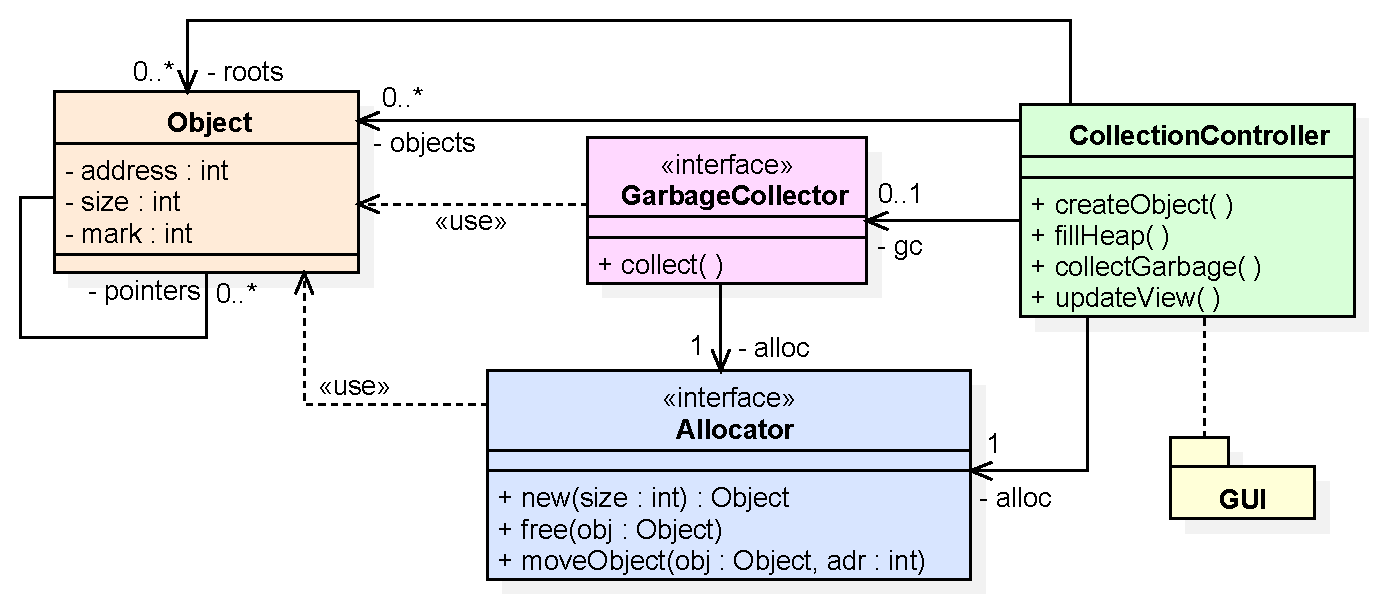
\includegraphics[scale=0.6]{img/uml/ch7-model.pdf}
	\caption[Klassendiagramm zur Modellierung von Mutator, Allokator und Kollektor]{Klassendiagramm zur Modellierung von Mutator, Allokator und Kollektor.}
	\label{fig:model}
\end{figure}

Heapobjekte werden als Instanzen einer Klasse \code{Object} modelliert und beinhalten Speicheradresse (\code{address}), Größe (\code{size}), Markierungsinformation (\code{mark}) und eine Menge \code{pointers} an Referenzen auf weitere Instanzen von \code{Object}, um die Menge \Pointers zu realisieren.
Ansonsten bieten sie keinerlei Funktionalität an.

Eine Instanz der Schnittstelle \code{Allocator} stellt die wesentlichen Dienste eines Allokators zu Verfügung.
Dazu zählt die Anforderung einer Speichermenge durch den Mutator mittels \code{new}, die Freigabe von Objekten und des durch sie belegten Speicherbereichs sowie das Verschieben eines Objekts.
Ersteres geschieht durch Übergabe der gewünschten Speichermenge und Rückgabe eines neu erzeugten Instanz von \code{Object}, die die entsprechende Speicheradresse enthält.
Der Allokator ist diejenige Instanz, die Informationen über den Füllstand des Heaps und insbesondere über die Belegung einzelner Wörter besitzt.
Die Schnittstelle \code{GarbageCollector} beschreibt die Funktionalität eines Kollektors, welche im Wesentlichen aus der Durchführung eines Garbage-Collection-Zyklus (Methode \code{collect}) besteht.
Da eine Garbage Collection die Freigabe und Verschiebung von Objekten auslösen kann, verwaltet sie genau eine Instanz von \code{Allocator}.
Die Klasse \code{CollectionController} realisiert einerseits die Aufgabe des Mutators, das heißt die Anforderung von Speicher für neue Objekte sowie die (Simulation von) Referenzmanipulationen, die zur Verwaisung von Objekten führen.
Daher besitzt sie zwei Mengen von Heapobjekten \code{objects} und \code{roots}.
\code{objects} enthält dabei sämtliche Objekte des Heaps und \code{roots}\ -- entsprechend der Menge \Roots -- alle Basisobjekte.
Zudem verwaltet sie eine \code{Allocator}-Instanz, um Speicher anfordern zu können, sowie eine \code{GarbageCollector}-Instanz zur Auslösung der Garbage Collection.
Andererseits fungiert \code{CollectionController} als Steuerklasse, um über die GUI eingehende Benutzerinteraktionen umsetzen und delegieren zu können.

Die Idee ist nun, beim Start des Simulators zunächst eine Instanz der Klasse \code{CollectionController} erzeugen.
Diese legt wiederum -- je nach ausgewählter Garbage Collection -- eine geeignete \code{Allocator}-Instanz sowie einen \code{GarbageCollector} an.
Letzterer bekommt dabei den zuvor erzeugten Allokator übergeben, sodass Kollektor und Steuerklasse auf denselben simulierten Heap zugreifen.

\section{Implementation}
\label{sec:implementation}

\cleardoublepage

\chapter{Fazit}
Zusammenfassen, was in dieser Arbeit passiert ist.
Und, dass es noch viel mehr gibt.
Und ob der Visualisierer etwas taugt oder nicht.
%!TEX root = ../thesis.tex
\cleardoublepage
\thispagestyle{empty}

\vspace*{4.0cm}
\begin{flushright}
	\thesispartlabelfont Anhang
	{\color{ctcolorpartline}%
				\hspace*{-200pt}\rule[45pt]{600pt}{2pt}}
\end{flushright}

\setcounter{chapter}{0}
\renewcommand\thechapter{\Alph{chapter}}
\addcontentsline{toc}{part}{Anhang}

%!TEX root = ../../thesis.tex
\chapter{Beispiel zur verborgenen Referenzzählung}
\label{cha:ulterior-example}

\todo[inline]{Beispiel einfügen}

%!TEX root = ../../thesis.tex
% Author: Phil Steinhorst, p.st@wwu.de

% --------------------------
% Back matter
% --------------------------
\addtocontents{toc}{\vspace{1em}}
{%
\setstretch{1.1}
\renewcommand{\bibfont}{\normalfont\small}
\setlength{\biblabelsep}{0pt}
\setlength{\bibitemsep}{0.5\baselineskip plus 0.5\baselineskip}
\printbibliography
}
\todo[inline]{Backtracking entfernen}

\vfill

Diese Masterarbeit wurde mit \LaTeXe unter Verwendung der Vorlage \textit{Clean Thesis} von Ricardo Langner gesetzt.
Für mehr Informationen siehe \url{http://cleanthesis.der-ric.de/}.

\chapter*{Abbildungsverzeichnis}
\addcontentsline{toc}{chapter}{Abbildungsverzeichnis}
\renewcommand\listfigurename{}
\vspace*{-2.35cm}
\listoffigures


%\chapter*{Algorithmenverzeichnis}
%\addcontentsline{toc}{chapter}{Algorithmenverzeichnis}
\renewcommand\listalgorithmname{Algorithmenverzeichnis}
%\vspace*{-2.35cm}
\listofalgorithms

\newpage
\renewcommand{\listoflistingscaption}{Listing-Verzeichnis}
\listoflistings

\cleardoublepage

% !TEX root = ../../thesis.tex
%
%************************************************
% Declaration
%************************************************
%\pdfbookmark[0]{Eigenständigkeitserklärung}{Eigenständigkeitserklärung}
\addcontentsline{toc}{chapter}{Eigenständigkeitserklärung}
\chapter*{Eigenständigkeitserklärung}
\label{sec:declaration}
%\thispagestyle{empty}

Hiermit versichere ich, dass die vorliegende Masterarbeit \textit{\thesisTitle} selbstständig verfasst worden ist, dass keine anderen Quellen und Hilfsmittel als die angegebenen benutzt worden sind und dass die Stellen der Arbeit, die anderen Werken -- auch elektronischen Medien -- dem Wortlaut oder Sinn nach entnommen wurden, auf jeden Fall unter Angabe der Quelle als Entlehnung kenntlich gemacht worden sind.

\vspace*{2cm}

\begin{minipage}{0.5\textwidth}
	\begin{flushleft} \large
		\underline{\hspace{6cm}} \\
		{\footnotesize (Ort, Datum)}
	\end{flushleft}
\end{minipage}
~
\begin{minipage}{0.5\textwidth}
	\begin{flushright} \large
		\underline{\hspace{6cm}} \\
		{\footnotesize (Unterschrift)}
	\end{flushright}
\end{minipage}\\[0.5cm]

%*****************************************
%*****************************************

%\clearpage
%\newpage
%\mbox{}
\end{document}
